\chapter{Antecedentes}

\section{Modelo Est\'andar}

El Modelo Est\'andar es el formalismo te\'orico-experimental que hasta el d\'{\i}a de hoy  describe con mayor precisi\'on las interacciones entre las part\'{\i}culas elementales y los diferentes tipos de fuerzas que experimentan entre las mismas. Los mayores desarrollos te\'oricos y descubrimientos experimentales que dieron forma al Modelo Est\'andar se tuvieron en la segunda mitad del siglo XX con el desarrollo de la Teor\'{\i}a Cu\'antica de Campo, fruto del esfuerzo de cient\'{\i}ficos de todo el mundo los cuales a partir de los modelos te\'oricos y observaciones experimentales construyeron una clasificaci\'on de las part\'{\i}culas en base a sus propiedades fundamentales como lo son la masa, la carga el\'ectrica, el esp\'{\i}n, entre otras. Dicha clasificaci\'on se muestra en la Figura~\ref{fig:ME}. Las part\'{\i}culas elementales est\'an divididas en dos categor\'{\i}as, los fermiones y los bosones, los fermiones est\'an a su vez divididos en quarks y leptones los cuales tienen un valor fraccional de esp\'{\i}n (1/2), adem\'as de que obedecen la estadistica de Fermi-Dirac y el principio de exclusion de Pauli. Los quarks son particulas elementales que constituyen a los hadrones, ya que debido al principio de confinamiento los quarks no pueden co-existir en estado libre.

Cuatro son las fuerzas fundamentales en la naturaleza, la fuerza electromagn\'etica, la d\'ebil, la fuerte y la gravitacional, el modelo est\'andar incluye las tres primeras, la gravitacional no esta incluida sin embargo su contribuci\'on en la f\'{\i}sica de part\'{\i}culas es despreciable si se compara por ejemplo con la fuerza electromagn\'etica (una raz\'on de $10^{36}$ en la escala de los Giga-electr\'on volts). El modelo est\'andar esta respaldado por una serie de observaciones experimentales, la mas reciente fue la observaci\'on de una nueva part\'{\i}cula cuyas propiedades son consistentes con el boson de Higgs~\cite{higgs}. Sin embargo aun existen fen\'omenos en la naturaleza que no pueden ser explicados dentro del formalismo del modelo est\'andar, ejemplo de ello es la naturaleza y composici\'on de la materia oscura.

\begin{figure}
\begin{center}
  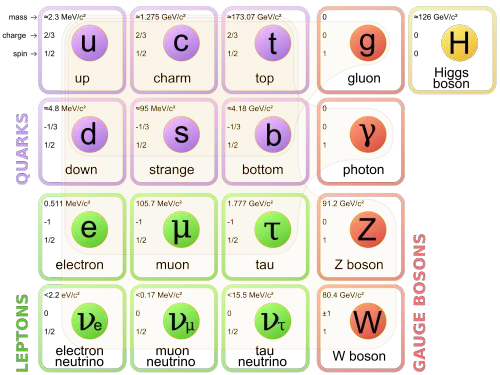
\includegraphics[width=4.0in]{standard-model.png}
  \caption{Clasificaci\'on de las particulas seg\'un el Modelo est\'andar de las part\'iculas elementales}
  \label{fig:ME}
\end{center}
\end{figure}


\section{Materia Oscura}

La materia oscura o dark matter (por su nombre en ingles) recibe este nombre debido a que no emite radiaci\'on electromagn\'etica, por lo que su existencia se infiere debido a su influencia gravitacional sobre la materia visible (o tambi\'en conocida como barionica) que se encuentra a su alrededor, dicho fen\'omeno ha sido observado en c\'umulos de galaxias en donde la velocidad de rotaci\'on de las mismas no corresponde a la que seria producida debido a la fuerza de gravedad ejercida por la materia visible a su alrededor. A pesar de los esfuerzos por parte de la comunidad cient\'{\i}fica hasta este momento se desconoce la composici\'on de la materia oscura, lo que se sabe, por medio de observaciones astron\'omicas, es que aproximadamente la materia oscura representa el 30.1\%  de la composici\'on materia-energ\'{\i}a del universo, el resto es energ\'{\i}a oscura (69.4\%) y materia visible (0.5\%). Recientemente y con el af\'an de entender la composici\'on de la materia oscura y su localizaci\'on en el universo la comunidad cient\'{\i}fica ha desarrollado varios experimentos, uno de los mas significativos es el Alpha Magnetic Spectrometer (AMS-02) el cual es un detector de part\'{\i}culas que tiene como uno de sus objetivos primordial el de buscar indicios de materia oscura, dicho detector fue dise\~nado y construido en el CERN para su futura instalaci\'on en la estaci\'on espacial internacional (ISS por sus siglas en ingles). Entre sus observaciones mas recientes~\cite{ams:cern} se ha reportado un flujo de positrones an\'omalo cuyo origen podria ser explicado por el proceso de aniquilaci\'on de part\'{\i}culas de materia oscura, donde en dicho proceso se libera energ\'{\i}a en forma de positrones .  Dicho flujo an\'omalo puede observarse a partir de los 25~GeV en la Figura~\ref{fig:AMS_positron} donde tambi\'en se presenta una comparaci\'on con otros experimentos que observan similar comportamiento.

\begin{figure}
\begin{center}
 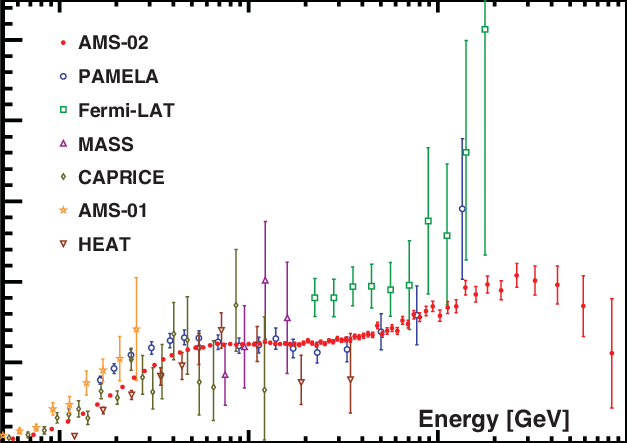
\includegraphics[width=4.0in]{AMS_positronflux.png}
  \caption{Flujo de positrones medido por el experimento AMS-02, comparado con los experimentos PAMELA,Fermi-LAT, MASS, CAPIRCE, AMS-01 y HEAT.}
 \label{fig:AMS_positron}
 \end{center}
\end{figure}

Dichas observaciones cosmol\'ogicas han motivado a los f\'{\i}sicos te\'oricos de altas energ\'{\i}as a postular nuevos modelos en los cuales la composici\'on de la materia oscura se pueda entender por medio de nuevas part\'{\i}culas elementales, las cuales no se encuentran descritas en el modelo est\'andar y que podr\'{\i}an estar siendo producidas en los aceleradores de part\'{\i}culas modernos como el Gran Colisionador de Hadrones en Ginebra, Suiza.  Dichos modelos propuestos entran en la categor\'{\i}a de extensiones al modelo est\'andar y por lo general involucran la existencia de nuevas part\'{\i}culas cuyas fuerzas e interacciones est\'an descritas por alguna variaci\'on de la Teor\'{\i}a Cu\'antica de Campo, lo que sugiere que sus mecanismos de producci\'on y propiedades pueden ser estudiadas por el formalismo de la f\'{\i}sica de part\'{\i}culas y la parte experimental por medio de los detectores de particulas lo cual involucra m\'etodos de recolecci\'on de datos, selecci\'on de eventos y t\'ecnicas estad\'{\i}sticas para extracci\'on de posibles se\~nales.

\section{Experimento CMS del CERN}

El experimento considerado en este proyecto es el Compact Muon Solenoid (CMS), el cual es uno de los detectores multi-usos del CERN, dicho detector tiene la capacidad de cubrir un amplio rango de procesos f\'{\i}sicos, como se comento anteriormente el CMS junto con el experimento ATLAS reportaron la observaci\'on de la part\'{\i}cula de Higgs en el 2012.  Este experimento consiste de varios subsistemas los cuales est\'an dise\~nados para la identifcaci\'on de pr\'acticamente todas las part\'{\i}culas del modelo est\'andar, para su dise\~no se tomo en cuenta como cada part\'{\i}cula interacciona con la materia, por ejemplo las part\'{\i}culas cargadas son identificadas por medio de detectores a base de silicio y de gas noble los cuales permiten determinar con precisi\'on el tiempo de cruce y localizaci\'on espacial de las part\'{\i}culas, adem\'as de que el signo de la carga es determinado deacuerdo a la deflecci\'on de su trayectoria debido al poderoso campo magn\'etico solenoide de 4 Teslas que envuelve al CMS.  Las part\'{\i}culas neutras son identificadas por la energ\'{\i}a que depositan en los calorimetros, la variedad de interacciones por tipo de part\'{\i}cula se puede ver en la Figura~\ref{fig:cms_interaction}. Los muones son part\'{\i}culas que interaccionan d\'ebilmente con la materia por lo que su detecci\'on se da un dos subsistemas, el detector de trazas, que corresponde a la primera capa de CMS y el sistema de muones, ultima capa del detector, lo cual permite una reconstrucci\'on de trayectoria muy precisa, debido a esto el posible decaimiento de las nuevas part\'{\i}culas a muones resulta un canal favorecido desde el punto de vista experimental.


\begin{figure}
\begin{center}
 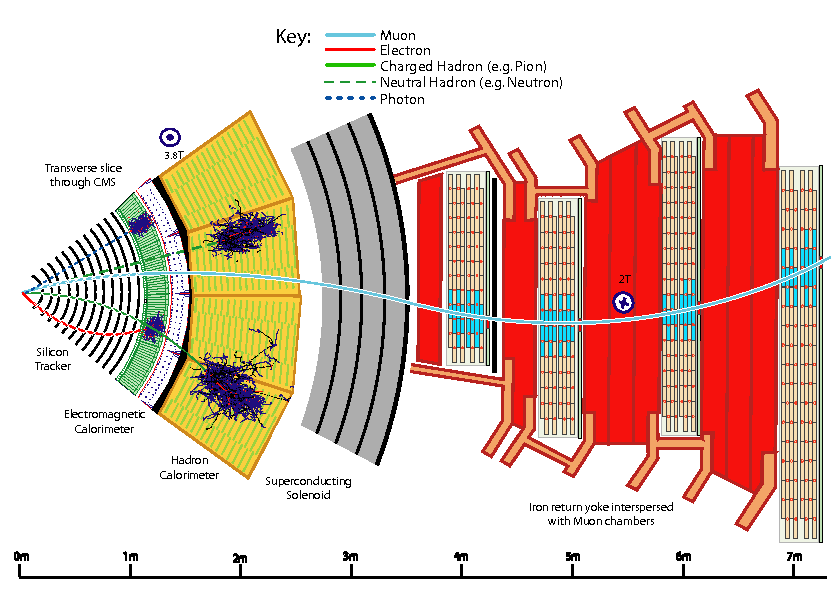
\includegraphics[width=4.0in]{cms_interaction.png}
  \caption{Representaci\'on de la interacci\'on de las part\'{\i}culas en el detector CMS del CERN}
 \label{fig:cms_interaction}
 \end{center}
\end{figure}

\chapter{Propuesta}

En este trabajo se propone hacer un estudio por medio de simulaci\'on de Monte Carlo de los modelos te\'oricos que predicen la creaci\'on de nuevas part\'{\i}culas como producto de la colisi\'on de protones altamente energ\'eticos. Estas nuevas part\'{\i}culas serian candidatas a explicar la composici\'on de la materia oscura.  Usualmente en dichos modelos las nuevas part\'{\i}culas interaccionan d\'ebilmente con el sector del modelo est\'andar, es decir con la materia visible por lo que su detecci\'on se dar\'{\i}a de forma indirecta, o en otras palabras, por su decaimiento a part\'{\i}culas conocidas del modelo est\'andar~\cite{Curtin2015} .  Adicionalmente al estudio de los modelos te\'oricos se pretende trabajar en la parte experimental, la cual consiste en el estudio, de igual manera por medio de simulaci\'on, de la respuesta del detector al paso de las part\'{\i}culas elementales y extracci\'on de los observables experimentales como los son la energ\'{\i}a de las part\'{\i}culas, el momento, la trayectoria, entre otros.  La parte experimental es fundamental ya que sin una buena estrategia de selecci\'on de datos, t\'ecnicas de supresi\'on de ruido y optimizaci\'on de la se\~nal seria imposible la observaci\'on de esta nueva f\'{\i}sica. En este proyecto se considera el detector CMS del CERN como el aparato experimental que proporcionara los datos de estudio, ya sea por simulaci\'on o por uso de datos reales.  

En una primera fase se pretende analizar los modelos te\'oricos de una manera fenomenol\'ogica, es decir por medio de paquetes de simulaci\'on propios del \'area de altas energ\'{\i}as, adem\'as de entender la respuesta del detector a las nuevas se\~nales, buscando optimizar la selecci\'on de los eventos en base a las propiedades de cada modelo, en una segunda fase se pretende estudiar la se\~nal de dichos modelos bajo diferentes escenarios del detector CMS, un primer escenario seria la configuraci\'on actual del detector CMS, que es la configuraci\'on usada hasta el 2018, durante el llamado periodo 'Run-2'' y comparar los resultados con el detector que se tiene propuesto para la fase de alta luminosidad o tambi\'en llamada Phase-2, la cual empezara  a partir del 2025, de esta manera se puede predecir en base a los estudios de simulaci\'on las posibilidades de identificaci\'on de una nueva se\~nal en los pr\'oximos a\~nos y como la actualizaci\'on de los detectores y m\'etodos de identificaci\'on de part\'{\i}culas podr\'{\i}an contribuir a incrementar las probabilidades de descubrimiento de estas nuevas part\'{\i}culas. 


\chapter{Justificaci\'on}

Los estudios de nueva f\'{\i}sica, en particular los que predicen la producci\'on de nuevas part\'{\i}culas son bastantes relevantes dado que se aproxima la etapa de alta luminosidad del gran colisionador de hadrones, en donde se lograra acumular datos con una frecuencia 10 veces mayor en la que actualmente se esta operando, es decir la probabilidad de detecci\'on de nuevas se\~nales sera mucho mayor ya que se lograra alcanzar un rango de energ\'{\i}a mayor y una cantidad de datos igualmente superior. Usualmente la probabilidad de producci\'on de estas part\'{\i}culas ex\'oticas es baja por lo que se requiere de una cantidad grande de datos para poder observar dicha producci\'on. El periodo de alta luminosidad esta programado para empezar a partir del a\~no 2024 o 2025 como se puede ver en al linea de tiempo del Gran Acelerador de Hadrones en la Figura~\ref{fig:lhctimeline} sin embargo desde este momento se esta trabajando en la actualizaci\'on del detector, m\'etodos de an\'alisis y estrategias que ayuden a optimizar la b\'usquedas de nueva f\'{\i}sica. 

\begin{figure}
\begin{center}
  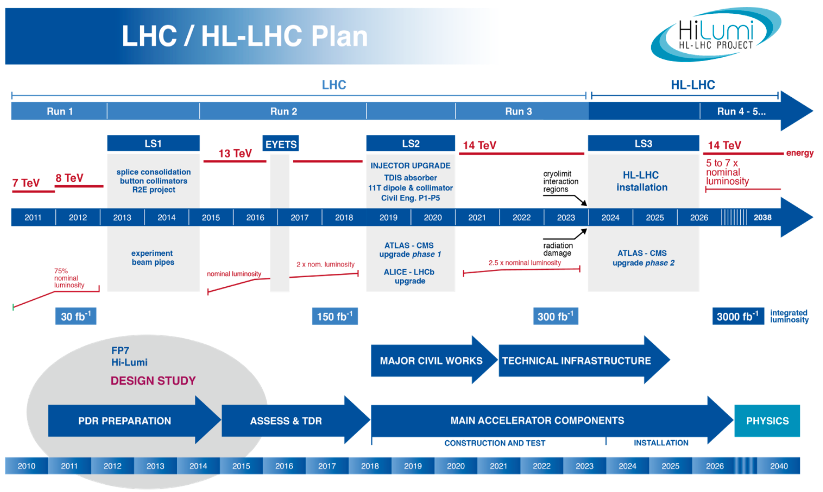
\includegraphics[width=4.0in]{lhc_timeline.png}
  \caption{Agenda de actividades del Gran Colisionador de Hadrones, donde la fase de alta luminosidad esta programada para iniciar a partir del 2024-2025}
  \label{fig:lhctimeline}
\end{center}
\end{figure}


Actualmente los modelos te\'oricos que predicen la formaci\'on de part\'{\i}culas de materia oscura no han sido explorados ampliamente, en gran medida por falta de datos experimentales que permitan alcanzar el espacio fase que dichos modelos predicen para esas part\'{\i}culas.  Actualmente con el funcionamiento del gran acelerador de hadrones y sus proyecciones en cuanto a recolecci\'on de datos en lo pr\'oximos a\~nos es la perfecta oportunidad para empezar a explotar lo mas posible el estudio de dichos modelos, para en dado caso descubir una nueva se\~nal sea f\'acil su interpretaci\'on en el contexto de alguno de los modelos propuesto.


\chapter{Hipotesis}

La hip\'otesis que se maneja en este estudio se basa en el estudio de modelos solidos que postulan que la materia oscura esta compuesta de part\'{\i}culas elementales, las cuales no han sido observadas hasta este momento, sin embargo podr\'{\i}an ser producidas en el laboratorio, de ser esto cierto se requiere de una marco te\'orico, es decir una teor\'{\i}a mas all\'a del modelo est\'andar que de sustento a dicha hip\'otesis. Afortunadamente ya existen varias modelos propuestos que predicen dicha producci\'on, uno de los modelos mas populares es el del llamado sector oscuro, o dark sector, por sus siglas en ingles, en el cual debido al rompimiento de una simetr\'{\i}a se da lugar a la producci\'on del llamado fot\'on oscuro (dark photon), dicha part\'{\i}cula seria la part\'{\i}cula portadora entre el sector oscuro y el del modelo est\'andar, es decir se comportar\'{\i}a como un boson, y la interacci\'on entre estos dos sectores se dar\'{\i}a por medio de lo que se conoce como el par\'ametro cin\'etico de mezcla (kinetic mixing parameter), usualmente abreviado como $\epsilon$~\cite{LB}, el cual mide la interacci\'on entre los dos sectores.

Una de las características de esta nueva part\'{\i}cula y que la diferencia del fot\'on del modelo est\'andar es que seria masiva y que su tiempo de vida podr\'{\i}a ser significativo, es decir en esta teor\'{\i}a esta nueva part\'{\i}cula tendr\'{\i}a dos par\'ametros libres (masa y tiempo de vida), adem\'as de que su deteccio\'on se dar\'{\i}a de forma indirecta, es decir por el decaimiento a part\'{\i}culas del modelo est\'andar.  Uno de los canales mas prometedores es en el que el fot\'on oscuro decae a muones. los muones son part\'{\i}culas que pueden ser identificadas y reconstruidas con gran eficacia usando el detector CMS por lo que la probabilidad de detecci\'on es mayor que con otros modos de decaimientos.

Adicionalmente en varios de estos modelos el boson de Higgs puede servir como portal del sector oscuro~\cite{Arcadi:2019lka}, es decir, existe la probabilidad de que uno de los decaimientos del boson de Higgs sea a part\'{\i}culas como el fot\'on oscuro, esto es valido para el boson de higgs del modelo est\'andar, es decir el recientemente observado y cuya masa es de 125~GeV, pero tambi\'en podr\'{\i}a encajar consistente con teor\'{\i}as que predicen mas de un boson de higgs, incluso con aquellos que postulan la existencia de part\'{\i}culas supersimetricas.




\begin{figure}
\begin{center}
  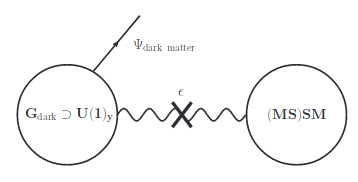
\includegraphics[width=2.8in]{sketch_darksector.png}
  \caption{Ilustracion esquem\'aticas de la conexi\'on entre el sector oscuro y el modelo estandar, los cuales est\'an conectados mediante un termino de mezcla din\'amica $\epsilon$}
  \label{fig:AMS_positron}
\end{center}
\end{figure}


\chapter{Objetivo General}

El objetivo general del proyecto es que se estudien, principalmente por medio de simulaci\'on, los diferentes modelos te\'oricos disponibles que predicen la creaci\'on de part\'{\i}culas de materia oscura en las colisiones de protones del experimento CMS del CERN.  Se buscara optimizar los par\'ametros de los modelos y t\'ecnicos experimentales que contribuyan a la b\'usqueda de dicha se\~nal en los pr\'oximos a\~nos.   Se pretende que dicho trabajo de simulaci\'on sirva de base para un trabajo futuro mas detallado donde se incorporen t\'ecnicas mas avanzadas de estudio. 


\chapter{Objetivos Especificos}

Se pretende alcanzar los siguiente objetivos especificos: 

\begin{itemize}
\item Entender los modelos teoricos que predicen la formaci\'on de part\'{\i}culas nuevas candidatas a dar explicaci\'on a la materia oscura, lo cual incluye ser capaz de variar los par\'ametros e incluir dichas variaciones en paquetes de simulaci\'on propios de la comunidad de altas energ\'{\i}as. 
\item Desarrollar un entorno de simulaci\'on el cual permita generar muestras estadisticas que incluyan la descripci\'on del modelo, generaci\'on de eventos y simulaci\'on del paso de part\'{\i}culas por el detector CMS. 
 \item Desarrollar un entorno de an\'alisis el cual permita estudiar los eventos simulados o experimentales, el an\'alisis incluye desde el acceso de datos, selecci\'on de eventos, tecnicas de supresi\'on de ruido y t\'ecnicas de an\'alisis de se\~nales. 
\item Comparar los resultados con diferentes configuraciones del detector CMS, se pretende comparar el detector actual con el dise\~no futuro en la fase de alta luminosidad, esto es posible por medio de simulaci\'on. 
  
\end{itemize}


\chapter{Metodolog\'{\i}a}

Para lograr alcanzar los objetivos deseados se pretende seguir la siguiente secuencia de actividades con el tiempo aproximado para cada una de ellas:

\begin{itemize}
  
\item Producci\'on de muestras de MonteCarlo (2 meses): Se espera producir muestras de simulaci\'on de monte carlo para cada proceso de la se\~nal y ruido, el numero de eventos a producir depende del tipo de proceso que se este estudiando y su secci\'on eficaz, a menor seccion eficaz mayor numero de eventos que se necesitaran producir, las muestras se espera se produzcan usando los recursos computacionales de la Universidad de Sonora. Dicho paso requiere del desarrollo de codigo para la distribuci\'on de las corridas de simulaci\'on en forma paralela usando el cluster ACARUS. Los paquetes de simulaci\'on que se usaran seran MADGRAPH~\cite{Alwall:2007st}, Pythia y Delphes~\cite{deFavereau2014}.

\item An\'alisis preliminar (2 meses): El estudiante debe desarrollar diferentes herrammientas de an\'alisis de datos, con el fin de acceder a los datos producidos en la simulaci\'on y extraer las variables de interes, comunmente dichas herramientas de an\'alisis consisten de codigos escritos en lenguaje C++ y python, de esta manera el estudiante dearrollara habilidad en la manipulaci\'on de muestras de datos. 

\item Optimizaci\'on de la selecci\'on de eventos (2 meses): Despues del acceso de dataos de simulaci\'on y variables de interes se procedera al estudio de la selecci\'on de eventos, la cual a grandes razgos consiste en seleccionar el conjunto de variables fisicas y valores los cuales puedan optimizar el proceso de se\~nal y reducir lo mas posible la contribuci\'on del ruido. 

\item An\'alisis estad\'{\i}stico (3 meses): Despues de la selecci\'on de eventos se realizara un estudio estad\'{\i}stico en el cual se extraeran el numero de eventos de se\~nal y ruido despues de la selecci\'on, de ahi se puede interpretar los resultados en base a indicadores estad\'{\i}sticos y concluir la probabibilidad de obsservaci\'on con datos recolectados en los siguientes a\~nos.

\item Escritura de Tesis (3 meses): Despues del an\'alisis estadistico se presentara los resultados con expertos del area buscando una retroalimentacion, al mismo tiempo se procedera a la escritura del trabajo de tesis. 

\end{itemize}
  
\chapter{Resultados Esperados} 

De este proyecto se espera obtener los siguientes resultados.

\begin{itemize}
\item Identificaci\'on de los modelos te\'oricos mas interesantes y cuyos parametros sean accesibles con la configuraci\'on del detector CMS, es decir la energia de colisi\'on y los eventos proyectados a recolectar en los proximos a\~nos, de esta manera se pretende acotar los diferentes modelos disponibles.
\item Imnplementaci\'on de un entorno de simulaci\'on, de una manera que sea practico y reutilizable por la colaboraci\'on para futuros estudios
\item Desarrollo de nuevas herramientas de an\'alisis que permitan incrementar la probabiliad de detecci\'on de este tipode se\~nales, es decir se buscara implementar algoritmos que contribuyan a la mejor identificaci\'on de part\'{\i}culas como el foton oscuro.
\item Mejorar los paquetes de simulaci\'on y an\'alisis experimental ya que actualmente no se encuentran optimizados para el estudio de particulas como el foton oscuro, que debido a sus propiedades particulares (tiempo de vida largo) y se requiere de implementaciones especiales en la parte experimental.
\end{itemize}




